\begin{strip}
\centering
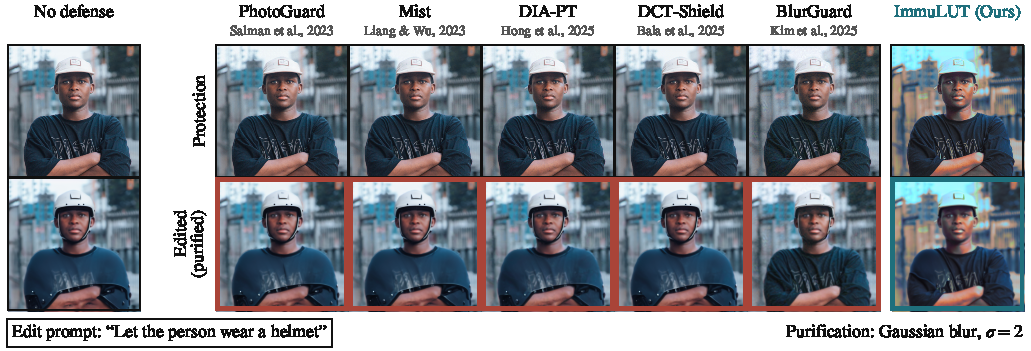
\includegraphics[width=\linewidth]{fig/teaser.pdf}
\captionsetup{hypcap=false}
\captionof{figure}{Protected images (top) and their InstructPix2Pix edits (bottom) with the instruction ``Let the person wear a helmet'' after Gaussian blur purification ($\sigma = 2$). While the additive defenses (red), including BlurGuard, fail to prevent the requested helmet insertion after purification, \capg{} (teal) successfully prevents the helmet from appearing, demonstrating its robustness to purification.}
\captionsetup{hypcap=true}
\label{fig:teaser}%
\end{strip}
